The parallel implementation for PFEM-2 follows the guidelines presnted in \cite{gimenez:parallel} for the case of distributed memory architectures. The challenges are well described in their paper but basically involves the extra amount of memory needed for the particle data structure. Due to the explicit scheme the parallel implementation needs to take care of local operations to each particle separately from the rest allowing for trivial parallelization. The dificulty arise at the interface between processors where particles may travel several elements and possible processors before finding their final host element. This task requieres an outer loop to communicate particles that will terminate when no more particles cross the interface between partitions. In figure \ref{fig:parallel} there is an illustration of how particles may move across processors. The thick black line depicts the partition. In the first case a particle lands in the same processor which involves no communication. In the second case a particle moves across a single interface and communication takes place. In the third place a particle may move accross two or more processors in which case the outer loop will perform as many communications as necessary untill no more particles cross a processor interface.

\begin{figure}[htp] 
\centering 
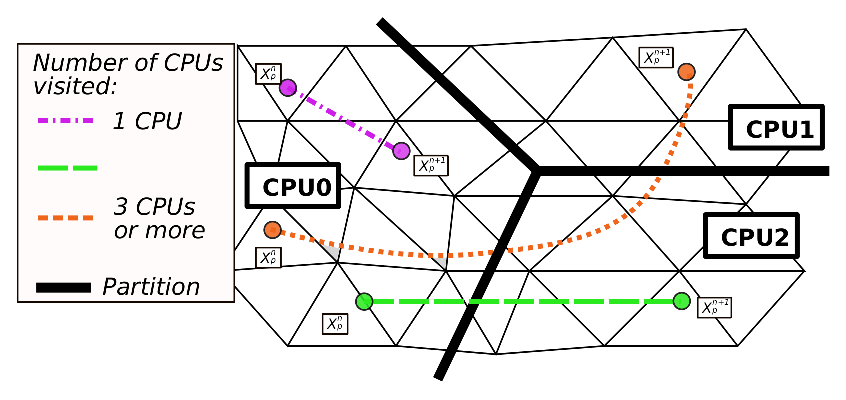
\includegraphics[scale=.4]{./imgs/parallel.eps}
\caption{Different ways that particles may move across processor interfaces.}
\label{fig:parallel}
\end{figure}


The current approach is built ``on top'' of a pre-existing parallel FEM implementation thus inheriting much of the data structures and methodologies. The partitions are creating using the software METIS \cite{metis1,metis}...

In the present implementation load balancing has not being address. Extrictely speaking if particles are not removed at some point accumulation of particles in one partition will be an issue. This is something that will be address later. Most luckily the PFEM-2 impliementation will change to allow removal of particles in such a way that an almost constant amount of particles is preserved at each element. The techniques for particle inventory presented in \cite{gimenez-difusion} will be implemented.



[IMAGE WITH PARTICLES MOVING THROUGH PARTITIONS]



[IMAGE SCALABILITY]


 
